\begin{figure}[!h]
\centering
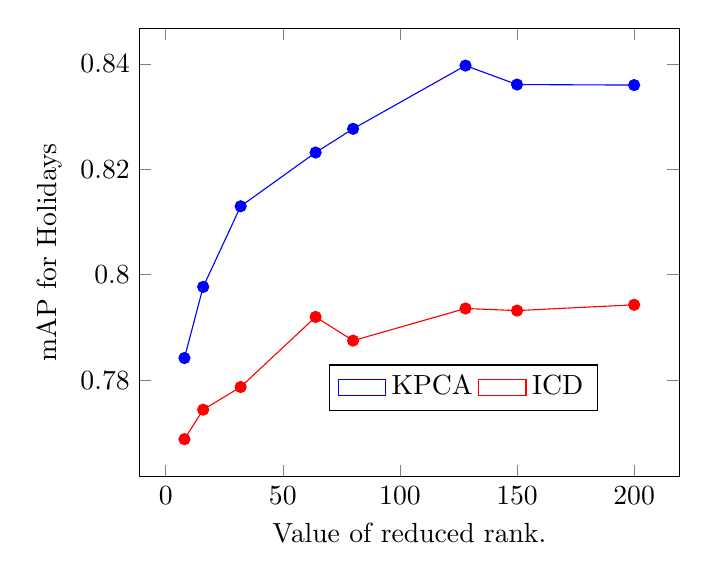
\begin{tikzpicture}
	\begin{axis}[
		xlabel=Value of reduced rank.,
		ylabel=mAP for Holidays,
		legend style={
			area legend,
			at={(0.6,0.25)},
			anchor=north,
			legend columns=-1}]
%%Poly SLEM
    \addplot[mark=*, blue] coordinates{
        (  8, 0.7842)
        ( 16, 0.7977)
        ( 32, 0.8130)
        ( 64, 0.8232)
        ( 80, 0.8277)
        (128, 0.8397)
        (150, 0.8361)
       ( 200, 0.8360)
    };
    \addlegendentry{KPCA}
    \addplot[mark=*, red] coordinates{
        (  8, 0.7688)
        ( 16, 0.7744)
        ( 32, 0.7787)
        ( 64, 0.7920)
        ( 80, 0.7875)
        (128, 0.7936)
        (150, 0.7932)
       ( 200, 0.7943)
    };
    \addlegendentry{ICD}
	\end{axis}
\end{tikzpicture}
\caption{mAP for Holidays using SPoC + Poly SLEM. We perform two low-rank decompositions and compare its results at similar ranks.}
\label{kpca:icd}
\end{figure}

